\documentclass{beamer}
\usetheme{metropolis}

\usepackage[utf8]{inputenc}
\usepackage[normalem]{ulem}
\usepackage{csquotes}

\title{IDU1321. Ettevõtte äriarhitektuur}
\subtitle{Neljas loeng}
%\date{10.09.2017}
\author{Andres Kütt}
\institute{Cybernetica, arhitekt}


\begin{document}

\begin{frame}
\titlepage
\end{frame}

\begin{frame}[standout]
Küsimusi loetu kohta?
\end{frame}


\begin{frame}[standout]
Küsimusi jagatud linkide kohta?
\end{frame}

\begin{frame}[standout]
Küsimusi kodutöö kohta?
\end{frame}

\begin{frame}[standout]
Tagasiside!
\end{frame}


\section{Äriprotsess ja kasutuslood}

\begin{frame}{Mis on äriprotsess?}
	\enquote{A business process or business method is a collection of related, structured activities or tasks that produce a specific service or product (serve a particular goal) for a particular customer or customers}

	Wikipedia
\end{frame}

\begin{frame}{Definitsioonist}
	\begin{enumerate}
		\item Kastid ekraanil ei ole äriprotsess. Tuletage meelde mudeli ja päris elu seoseid
		\item Äriprotsessil on eesmärk
		\begin{itemize}
			\item Eesmärgistamine on \emph{väga} keeruline, toote ja teenuse definitsioon samuti
			\item Kui asjal on lõpp, on tal ka algus
		\end{itemize}
		\item Äriprotsessil on klient
		\begin{itemize}
			\item Järelikult äriprotsess loob väärtust
			\item Kliendi leidmine võib osutuda mittetriviaalseks
		\end{itemize}
		\item Tegevustel on oma sisemine struktuur, protsessi sammud võivad samuti protsessid olla
	\end{enumerate}
\end{frame}

\begin{frame}{Notatsioonist}
	Mõned näited, tuletage meelde juttu kommunikatsioonist
	\begin{itemize}
		\item BPMN
		\begin{itemize}
			\item Mõeldud äriprotsesside uurimiseks
			\item Selgelt suunatud mittetehnilistele inimestele
			\item Võimaldab teha keerulisemaid asju
		\end{itemize}
		\item UML Activity Diagram
		\begin{itemize}
			\item Mõeldud tarkvara tootmiseks
			\item UMLi on suunatud arendajale
			\item Selgem semantika
		\end{itemize}
		\item Steven Spear
		\begin{itemize}
			\item UMLi \emph{Communication Diagram} ainult et inimestega
			\item Suunatud optimiseerimisülesannete lahendamisele
		\end{itemize}
	\end{itemize}
\end{frame}

\begin{frame}{Definitsioon}
	Kasutuslugu kirjeldab millegi tegemise detaile
	\begin{itemize}
		\item Eri määratlusi ja formaate on väga palju
		\begin{itemize}
			\item Ärge eeldage midagi, inimesed arvavad erinevalt
			\item Ainus hea põhjus formaadis kinni olla on kommunikatsioon
		\end{itemize}
		\item \emph{Use case}
		\begin{itemize}
			\item Kirjeldab \emph{programmi} tegevusi
			\item Klassikalisem, pikem ja paremini struktureeritud
			\item RUPi mall on suhteliselt levinud
		\end{itemize}
		\item \emph{Customer story}
		\begin{itemize}
			\item Kirjeldab \emph{kasutaja} tegevusi
			\item Lõdvema struktuuriga ja lühem
			\item Võib kergesti kirjeldada äriprotsessi üht lõime
		\end{itemize}
	\end{itemize}
\end{frame}

\begin{frame}[fragile]
	\begin{center}
		\LARGE{\textbf{Äriprotsessi mudelit võib vaadata arhitektuurina, kasutuslugusid konkreetsete osiste disainina}}
		\\[4cm]
		\small{Esimene on pigem suunatud arhitektile ja teine pigem programmeerijale. \textbf{NB!} Tuletage meelde, mis me rääkisime sotsiotehnilistest süsteemidest!}
	\end{center}
\end{frame}

\begin{frame}[fragile]
	\begin{center}
		\LARGE{\textbf{Kasutusloo ja tegevuse vahel võib olla mitu-mitmele seos}}
		\\[4cm]
		\small{Autentimine ja logimine, näiteks. Kõik sõltub kasutusloo määratlusest}
	\end{center}
\end{frame}


\begin{frame}{Tüüpilised äriprotsessi vead}
		\begin{itemize}
			\item Ebaühtlane ja/või liigne detailsus. Pea rangelt kinni $5\pm2$ reeglist
			\item Katse peegeldada mittelineaarsust
			\item Sisendi, väljundi või actorita sammud
			\item Mitme väljundiga sammud
			\item Segamini hägusa ja selge semantikaga elemendid 
			\item Kõigi tegevuste kõigi kombinatsioonide läbimine ei anna eesmärgiks seatud tulemust
			\item Kirjeldamata veasituatsioonide harud
		\end{itemize}
\end{frame}

\begin{frame}{Tüüpilised kasutuslugude vead}
		\begin{itemize}
			\item Liigne detail. Kes on kasutaja ja kui palju detaili ta vajab?
			\item Harude puudumine
			\begin{itemize}
				\item \enquote{Happy day} stsenaariumiga kaugele ei sõida
				\item Kui harusid on liiga palju, on protsessidiagramm liig kõrgel tasemel
			\end{itemize}
			\item Kõikuv formaat ja semantika
			\begin{itemize}
				\item Projekti lõpuks loksuvad ootused paika
				\item Kust teab lugeja, milline formaat \enquote{õige} on?
			\end{itemize}
			\item Keskendumine ilmselgele
			\begin{itemize}
				\item Kirjutame (detailselt) üles asjad, mida me teame
				\item Mida me ei tea või ei taha otsustada, kirjeldame ebamääraselt
				\item Mida progremmeerija vajab?
			\end{itemize}
		\end{itemize}

\end{frame}


\section{Harjutus}

\begin{frame}{Teeme makseid}
Modelleerige makse tegemise protsess internetipangas
\begin{itemize}
	\item Määratlege 
		\begin{itemize}
			\item protsessi algus ja lõpp
			\item klient
		\end{itemize}
	\item Tegutsege paarides
	\begin{itemize}
		\item 20 minutit tööd mudeli kallal
		\item 7 minutit esitlete oma tööd kõrvalpaarile
		\item 7 minutit kuulate nende tulemusi
	\end{itemize}
\end{itemize}
\end{frame}


\begin{frame}{Harjutuse kokkuvõte}
	\begin{itemize}
		\item Kas õnnestus tüüpilisi vigu vältida?
		\item Mida on veel vaja, et siit kasutuslugudega edasi minna? 
	\end{itemize}
\end{frame}

\begin{frame}[fragile]
	\frametitle{Organisatsiooni arhitektuur}

	\begin{center}
	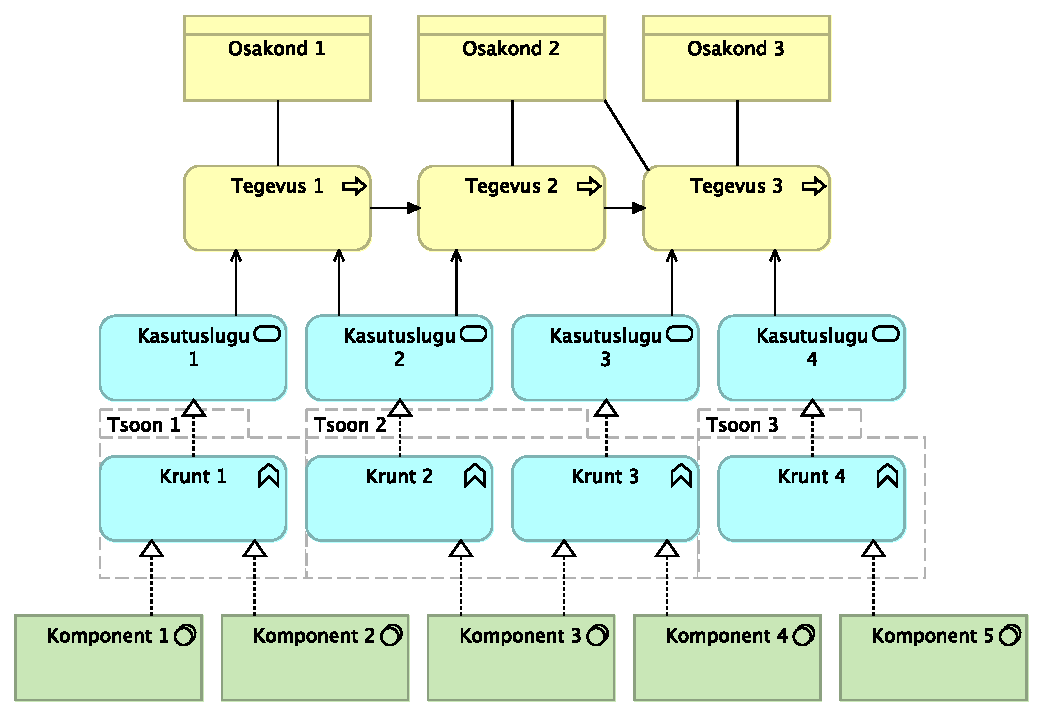
\includegraphics[width=.9\textwidth]{kihid.pdf}
	\end{center}
\end{frame}


\begin{frame}{Kordame}
	\begin{itemize}
		\item Äriprotsess on mudel, kasutuslugu on juhend
		\item Äriprotsess kirjeldab päris maailma, kasutusloo põhjal kirjutatud kood peab selles hakkama saama
		\item Modelleerides ärge unustage teada teadmatust
		\item Iga rida dokumentatsiooni on kohustus tuleviku ees
	\end{itemize}
\end{frame}

\begin{frame}{Järgmine kord}
\begin{itemize}
	\item Linnaplaneerimine
	\item Kasutuslood ja linn
	\end{itemize}
\end{frame}

%\begin{frame}{Bibliography}
%	\bibliographystyle{plainnat}
%	\bibliography{idu1321}
%\end{frame}

\begin{frame}[standout]
Küsimusi?
\end{frame}

\end{document}
